\section{The \AC{} Approach}
\label{sec:ac_argoncube}

To address the challenges mentioned in Section~\ref{sec:lartpc_challenges}, the \gls{help} group has formed the \AC{} collaboration, with the goal of developing a new fully-modular type of \lartpc{}.
Modularity reduces pile-up and allows for shorter drift-times, thus slackens the requirements on argon purity and \gls{hv}.
A modular detector also contains light within each module, allowing for a more accurate trigger system.
Maintenance and upgrading of a modular detector is much easier than for a monolothic one.


\subsection{Modularity}
\label{sec:ac_argoncube_mod}

\AC{} is made of self-contained \gls{tpc} modules sharing a common cryostat.
In case of a fault condition the affected module(s) can be shut down and repaired or replaced individually without affecting the rest of the detector.
During construction, one can start data taking as soon as the first module is operational and needs not wait for the commissioning of the whole detector.
A modular detector furthermore reduces event pile-up because the acquisition time is reduced to the size of one half module.
This is crucial in the high-multiplicity environments of future \lar{} neutrino detectors.
Finally, also trigger purity profits from a modular approach because scintillation light is contained within each module, allowing for a localised trigger.

\begin{figure}[htb]
	\centering
	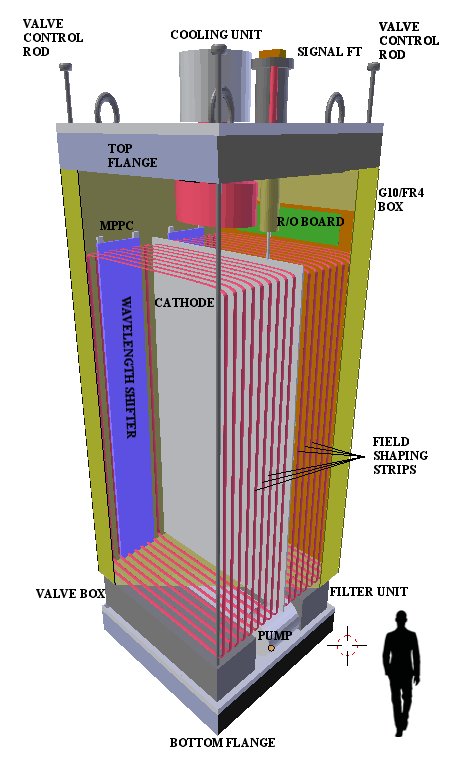
\includegraphics[height=.5\textheight]{ac/module}
	\caption[\AC{} module schematic]{%
		Schematic of an \AC{} module.
	}
	\todo[inline]{better, more recent picture}
	\label{fig:ac_module}
\end{figure}

A module is made of a rectangular box with a square footprint and the height required by physics goals and/or sensitivity constraints.
The top and bottom flanges are made of stainless steel while the side walls are made from \SI{1}{\centi\metre} G10 sheets.
G10 is a glass-reinforced epoxy composite formerly used for \glspl{pcb}.
Its low density makes it more transparent for passing particles allowing for a performance comparable to a monolithic detector.
At the same time, the dead volume is drastically reduced compared to a monolithic design due to the comparably low cathode voltage (see Section~\ref{sec:dune-nd_ac}).
The modules are placed side-by-side in a bath of \lar{} where they can be extracted and reinserted as needed.
Pressure inside the modules is kept close to the bath pressure putting almost no hydrostatic force on the module walls.
Purity of the \lar{} is maintained within each module by means of a recirculation system (see Section~\ref{sec:ac_argoncube_cryo}).
As a result, the argon surrounding the modules needs not meet as stringent purity requirements as the argon inside.
Under normal operation conditions, all modules are inserted with only clearance distances between modules, and their top flanges sealed using indium.
The schematic of an \AC{} module is shown in Figure~\ref{fig:ac_module}.

To extract a module, the indium seal around the flange in question is removed.
The module is then slowly lifted up by a crane and the \lar{} is drained to the surrounding bath through a hydrostatic outlet valve at the bottom of the module by means of gravity.
On the bottom of the module, a blind flange is located with equal dimensions as the top flange but without any feedthroughs.
When the bottom flange reaches the original position of the top flange, it is sealed with indium again and then detached from the module which is now free and can be brought to its destination.
Upon reinsertion, the procedure is reversed.
First, the module is reattached to the blind flange and the indium seals is removed.
Then, it is slowly inserted into the argon bath while being filled through a hydrostatic inlet valve at the bottom of the module by means of hydrostatic pressure.
As soon as the top flange of the module reaches the top flanges of the other modules, the indium seal is reinstalled.
Figure~\ref{fig:ac_module-ins-ext} shows the insertion (left) and extraction (right) of a module, for the \num{2 x 2} prototype at \gls{help} (see Section~\ref{sec:dune-nd_ac_2x2}).

\begin{figure}[htb]
	\centering
	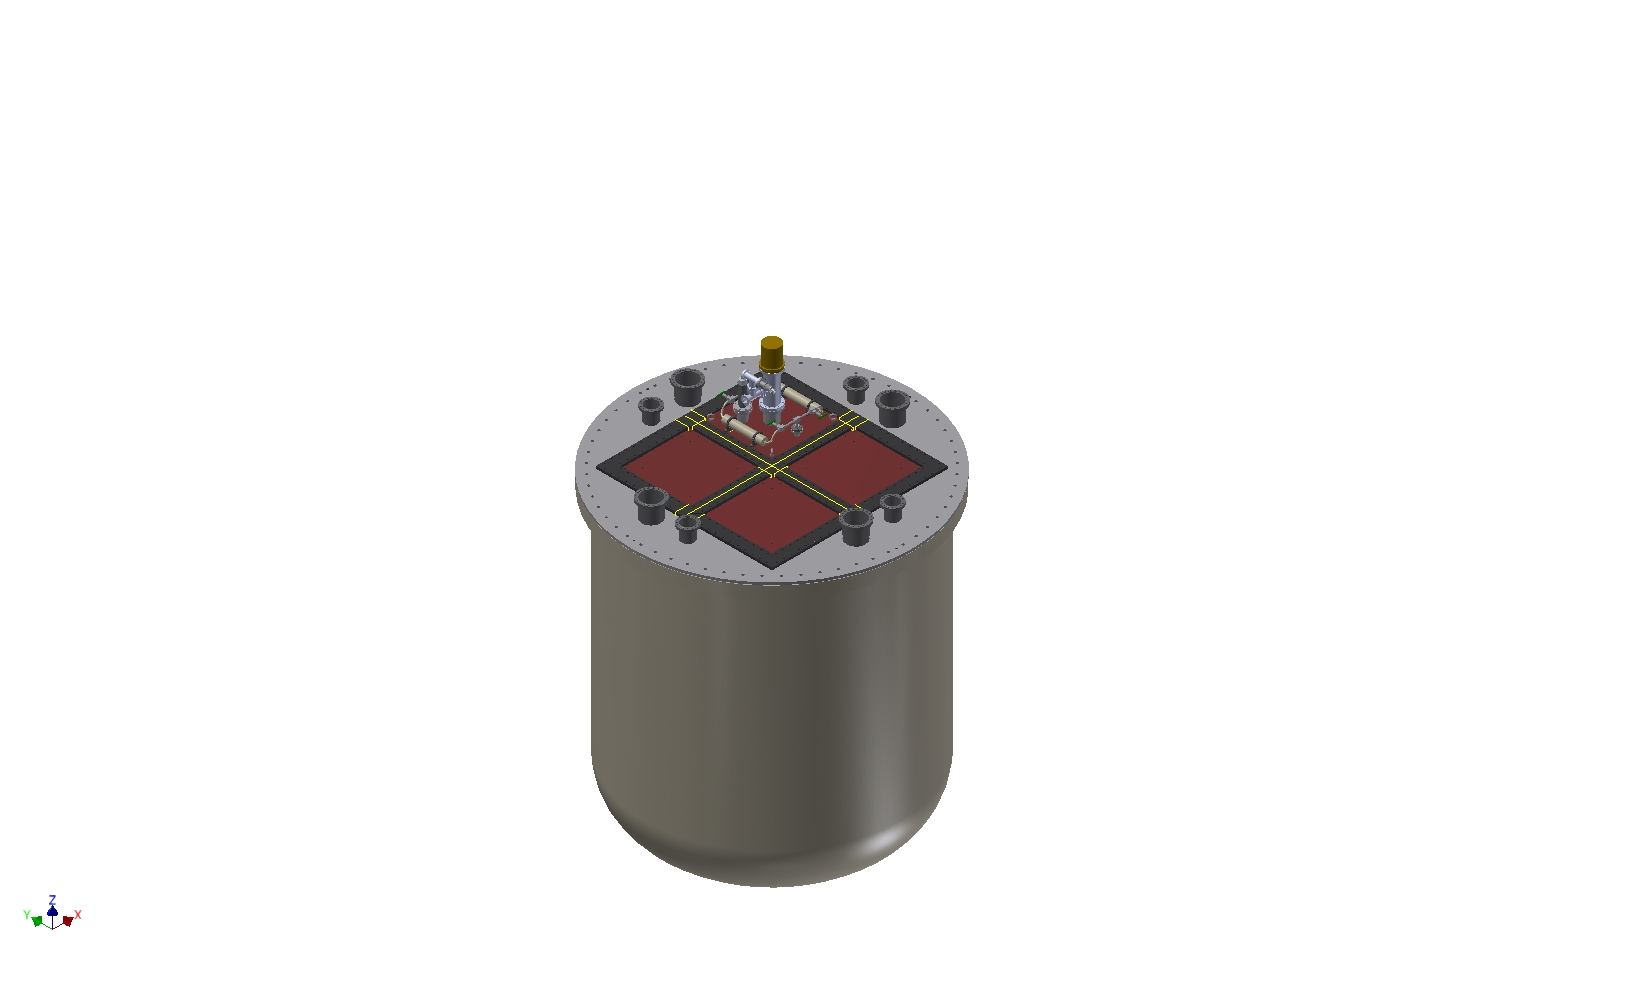
\includegraphics[viewport=500 90 1000 700, clip, width=.495\textwidth]{ac/2x2/module_inserted}
	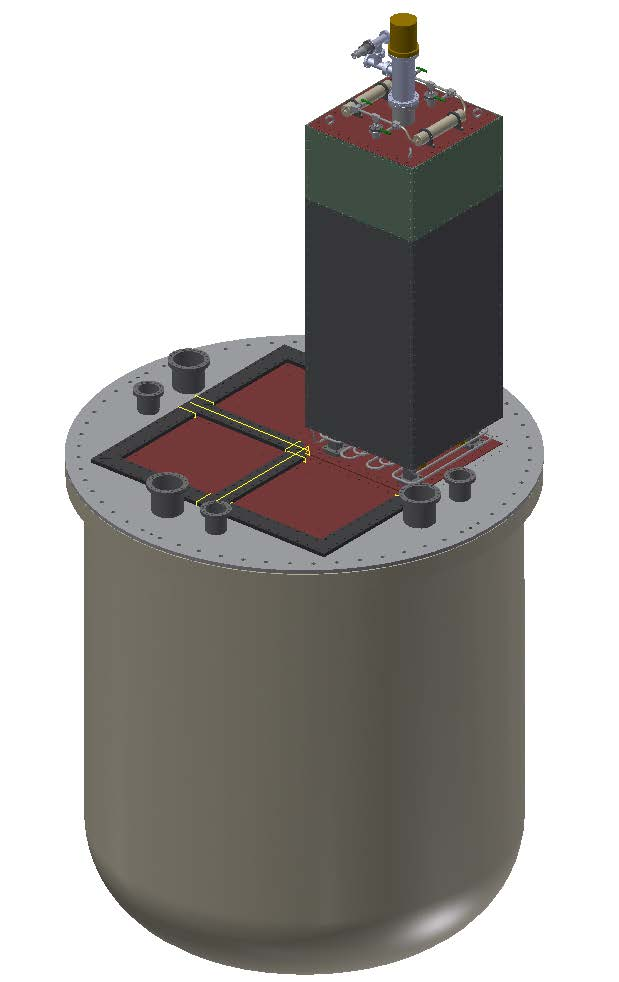
\includegraphics[width=.495\textwidth]{ac/2x2/module_extracted}
	\caption[\AC{} module insertion and extraction]{%
		Inserted (left) and extracted (right) module.
	}
	\label{fig:ac_module-ins-ext}
\end{figure}

\subsection{Drift Field Generation}
\label{sec:ac_argoncube_hv}

Another big problem that can be solved by a modular \gls{tpc} design are the high electric fields required for large detectors, and the resulting stored energy.
Because each module contains its own \glspl{tpc} independent of all other modules, the required cathode potential only depends on the module size not the detector size.
To minimise the cathode voltage, the field is applied along one of the short edges of a module and furthermore, the module is split in half by the cathode reducing the voltage by another factor of two.
Thus, for a module footprint of \SI{1 x 1}{\metre} and an electric field of \SI{1}{\kilo\volt\per\centi\metre}, a cathode potential of only \SI{50}{\kilo\volt} is required.
Operating a \lartpc{} at this voltage is challenging but feasible without a prohibitive loss in fiducial volume~\cite{AT}.
The \gls{hv} is brought into the module using a feedthrough similar to the one used for the breakdown studied presented in Section~\ref{sec:studies_hv}.
Due to the moderate cathode voltage, commercial alternatives are also available.
Using conventional \gls{pcb} techniques, field-shaping rings can be realised as copper traces directly printed onto the G10 module walls.
They are connected via high-voltage resistors in the same fashion as for a classic \lartpc{}.
An improved solution with a continuous resistive-plane field cage is under investigation.
This could provide a very homogeneous field paired with simple mechanics.
The difficulty is to find a material with the required sheet resistivity of $\sim{\SI{1}{\giga\ohm\per sq}}$\footnote{Sheet resistivity only depends on the aspect ratio of the sheet but not its area. It is therefore quantified as a resistance per square.} that is stable at cryogenic temperatures and deposable on G10.


\subsection{Cryogenics}
\label{sec:ac_argoncube_cryo}

During module insertion and extraction, the argon flow is controlled by hydrostatic check valves located at the bottom of the module.
They require a minimal differential pressure to open.
Purity inside to modules is maintained by means of continuous \lar{} recirculation through oxygen traps.
The dirty argon is sucked in at the module top and then pushed through the oxygen traps.
The clean argon is first routed through a heat exchanger located below the module inside the outer bath for cooling, and then re-enters the module at the bottom.
For optimal heat transport, the argon flow is directed along the cold electronics.
To prevent dirty argon from the bath entering the modules, their interior is held at a slight overpressure, just below the opening pressure of the check valves.
Cooling power to the bath is supplied by cryocoolers located in unistrumented volumes at the side of the detector called service volumes.

There are two slightly different options for the recirculation system.
To maximise module autonomy, each module can be equipped with its own oxygen trap and \lar{} pump.
One drawback of this is the very high cost of \lar{} pumps.
Currently, the \dune{} \gls{nd} complex is planned to consist of a magnetised detector besides an unmagnetised \lartpc{}.
The resulting magnetic stray fields might interfere with the electric motors of \lar{} pumps on top of the modules.
Using a shared recirculation circuit is more economic but reduces module autonomy.
The external system, comprising pump and oxygen traps, can be located outside the argon bath (and potential magnetic stray fields) connected to the modules via tubes.


\subsection{Charge Readout}
\label{sec:ac_argoncube_charge-ro}

The high rates present in a \gls{nd} environment will lead to a significant amount of event pile-up.
Disentangling the individual neutrino events requires a highly capable charge readout.
Solving this task with a projective wire readout is more than doubtful.
To enable true \gls{3d} tracking, the modules are equipped with a pixelated charge readout very similar to the one described in Section~\ref{sec:studies_charge-ro_pixel}.
Pixelated anode planes are located on the two outer walls parallel to the cathode.
To achieve unambiguous \gls{3d} information, the bespoke \pixlar{} cryogenic electronics described in Section~\ref{sec:studies_electronics_pixel} are used to digitise the signals in cold.


\subsection{Light Readout}
\label{sec:ac_argoncube_light-ro}

One of the main challenges for the light readout are again the high rates faced by a \gls{nd}.
To get proper timing for the third spatial coordinate, scintillation signals need to be correctly matched to charge signals (flash matching).
Furthermore attenuation due to Rayleigh scattering becomes a problem for large detectors (see Table~\ref{tab:lartpc_larprop}).
Both problems are greatly alleviated by using an opaque cathode and module walls, containing the scintillation light inside a single module half (\gls{tpc}).
Therein, pile-up is reduced due to the smaller volume.
Having a position-resolving light readout helps as well.
However, a modular \gls{tpc} introduces a new challenge: The dead spaces in between adjacent \glspl{tpc} have to be kept to a minimum because they introduce gaps in the recorded event topologies accompanied by lost energy.
Classic \glspl{pmt} could therefore only be mounted at the top and/or bottom of the module but this would still waste active argon volume.
Additionally, the light would be collected at the far ends of a long narrow volume.
Finally, due to their operating principle, \glspl{pmt} do not work well in high electric fields present near the field cage at the module top and bottom.
Therefore, \AC{} modules are instrumented with the \AL{} light collection system described in Section~\ref{sec:studies_light-col_al}.
With its light trap design, it  allows light collection from a large area with a minimal dead volume.
The location of the \glspl{sipm} at the edges of a dielectric sheet makes most of the light detector immune to electric fields.
Splitting \AL{} into several horizontal strips stacked vertically gives some spatial resolution in the vertical direction.
\AL{} sheets are mounted in between cathode and anode, parallel to the field cage, with the \glspl{sipm} directly attaching to the charge readout \gls{pcb}.
The additional dead volume of a few \si{\milli\metre} is similar to the one caused by the charge readout \glspl{pcb} in perpendicular direction.